% ~6 pages
\subsection{Multipath Propagation and Doppler Effects}

The performance of wireless communication systems is strongly affected by the physical propagation environment. In practice, wireless signals rarely propagate through a single ideal path. Instead, they are influenced by surrounding objects, user mobility, and the relative motion between transmitters, receivers, and scatterers. Among these effects, multipath propagation and Doppler effects are particularly important because they determine how the wireless channel varies over time and frequency.

In high-mobility scenarios such as vehicular communications, high-speed railways, unmanned aerial vehicles, and low-earth-orbit satellite links, these effects become more severe. Multipath propagation causes the transmitted signal to arrive at the receiver through multiple paths with different delays, while Doppler effects introduce frequency shifts and time variation. These two phenomena provide the basis for understanding doubly selective channels, which are one of the main motivations for advanced waveform designs such as OTFS.

\begin{figure}[H]
    \centering
    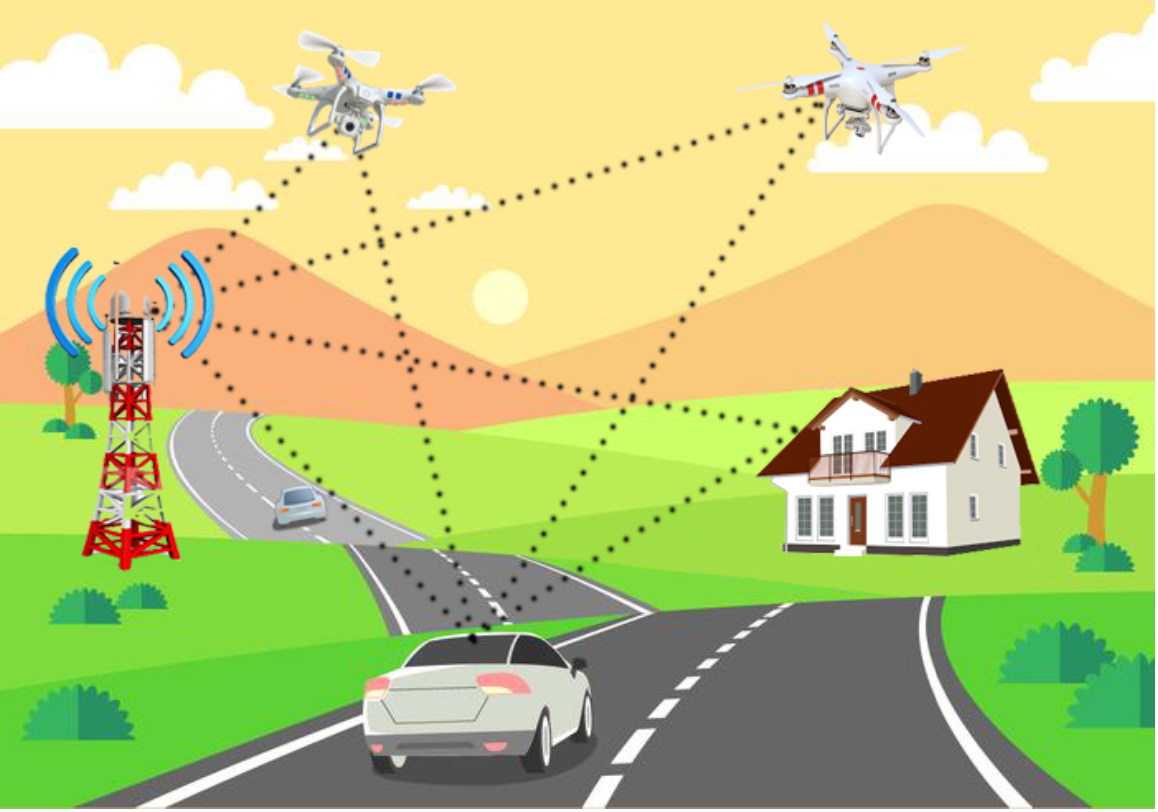
\includegraphics[width=0.82\textwidth]{Images/Chapter2/high_mobility_multipath.png}
    \caption[High-mobility wireless communication scenario with multiple propagation paths.]{High-mobility wireless communication scenario with multiple propagation paths~\protect\cite{Hong2019OTFSTutorial}.}
    \label{fig:high_mobility_multipath}
\end{figure}

Figure~\ref{fig:high_mobility_multipath} illustrates a high-mobility wireless communication scenario in which several terminals and reflecting objects coexist. The transmitted signal may reach the receiver through direct, reflected, diffracted, and scattered paths. Such a propagation environment leads naturally to both delay dispersion and Doppler dispersion.

\subsubsection{Multipath Propagation}

Multipath propagation occurs when transmitted electromagnetic waves reach the receiver through more than one propagation path. These paths may be created by reflection from buildings, diffraction around obstacles, and scattering from irregular objects such as trees, vehicles, and terrain. As a result, the receiver observes several replicas of the transmitted signal rather than a single clean copy.

Each propagation path is generally associated with a different path length. Therefore, the corresponding received signal component has its own delay, amplitude attenuation, and phase shift. The received waveform is formed by the superposition of all these components. Depending on their relative phases, the multipath components may combine constructively or destructively, causing fluctuations in the received signal strength.

A simple multipath channel can be represented as

\begin{equation}
h(t,\tau)=\sum_{i=1}^{P}h_i(t)\delta(\tau-\tau_i),
\end{equation}

where \(P\) is the number of propagation paths, \(h_i(t)\) is the complex channel gain of the \(i\)-th path, and \(\tau_i\) is the propagation delay of that path. This equation only states that the channel is composed of several delayed copies of the transmitted signal.

Figure~\ref{fig:high_mobility_multipath} illustrates the basic idea of multipath propagation. In addition to a possible direct path between the transmitter and receiver, the signal may also arrive through reflected or scattered paths. These additional paths usually travel longer distances and therefore arrive later than the direct component.

Multipath propagation is important because it directly affects the received signal quality. If the delayed components arrive within a short time interval, they may simply cause fading. However, if the delay differences are comparable to the symbol duration, different symbols may overlap at the receiver. This effect is known as inter-symbol interference (ISI).

Although multipath propagation is often considered a source of distortion, it may also provide diversity. Since different propagation paths carry different versions of the transmitted signal, a properly designed receiver can exploit these components to improve reliability. Modern wireless systems use equalization, coding, diversity combining, and multicarrier modulation to reduce the negative effects of multipath and, when possible, benefit from the available path diversity.

In the context of this thesis, multipath propagation is important because it leads to delay spread and frequency selectivity. These concepts are discussed in the next subsection.

\subsubsection{Delay Spread and Frequency Selectivity}

Delay spread is a direct consequence of multipath propagation. Since different propagation paths have different lengths, their corresponding signal components arrive at the receiver at different times. The difference between the earliest and latest significant arriving components is commonly referred to as delay spread.

The propagation delay of a signal path is proportional to the path length and can be expressed as

\begin{equation}
\tau=\frac{d}{c},
\end{equation}

where \(d\) is the propagation distance and \(c\) is the speed of light.

\begin{figure}[H]
    \centering
    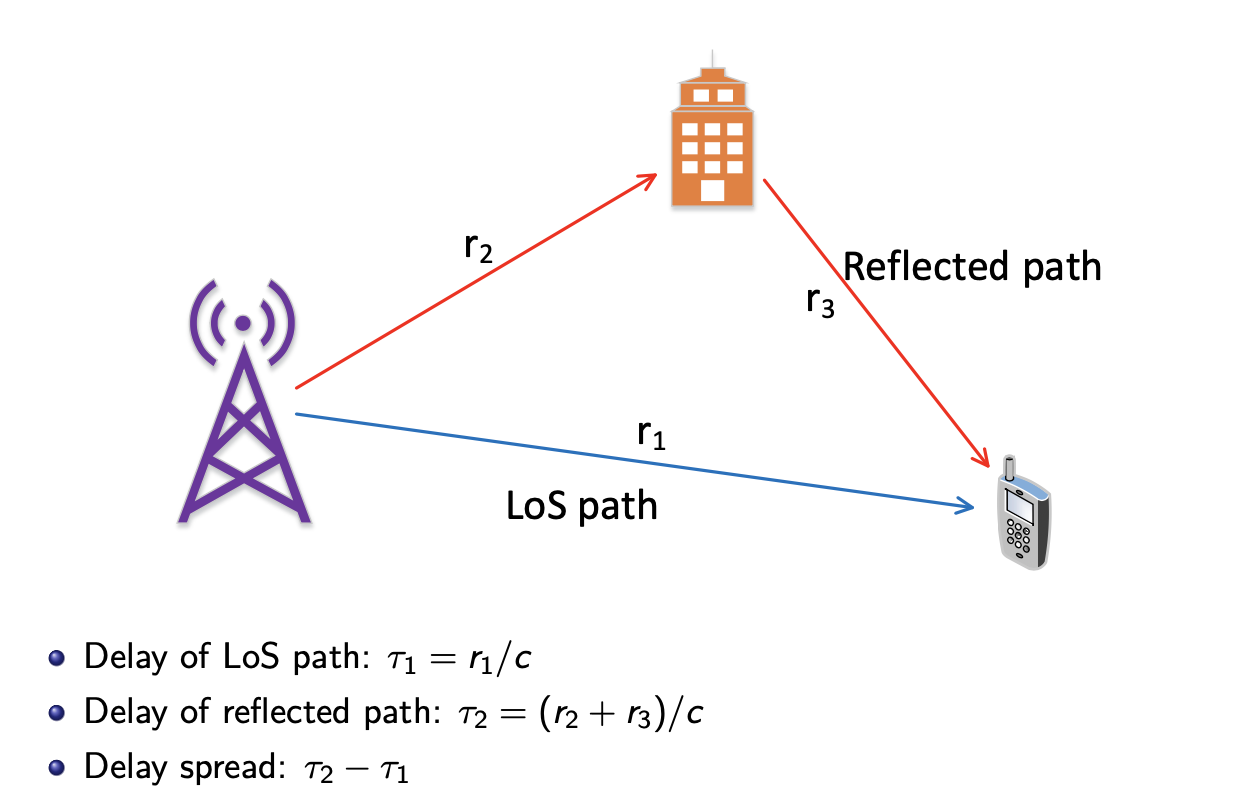
\includegraphics[width=0.82\textwidth]{Images/Chapter2/delay_spread.png}
    \caption[Illustration of delay spread caused by LoS and reflected propagation paths.]{Illustration of delay spread caused by LoS and reflected propagation paths~\protect\cite{Hong2019OTFSTutorial}.}
    \label{fig:delay_spread}
\end{figure}

Figure~\ref{fig:delay_spread} shows a simple example of delay spread. The direct Line-of-Sight (LoS) path travels a distance \(r_1\), while the reflected path travels through two segments with distances \(r_2\) and \(r_3\). Therefore, the corresponding delays can be written as

\begin{equation}
\tau_1=\frac{r_1}{c},
\qquad
\tau_2=\frac{r_2+r_3}{c}.
\end{equation}

The delay spread in this simple case is the difference between these two delays. A larger delay spread means that the received signal components are more spread out in time.

Delay spread has an important effect on the frequency-domain behavior of the channel. When a channel introduces significant delay dispersion, different frequency components of the transmitted signal may experience different attenuation and phase rotation. In this case, the channel is called frequency selective.

If the signal bandwidth is small compared with the frequency range over which the channel response is approximately constant, the channel behaves like a flat-fading channel. In a flat-fading channel, all frequency components of the signal are affected in nearly the same way. Conversely, when the signal bandwidth is large, different frequency components may experience different channel gains. The channel then becomes frequency selective.

Frequency selectivity is a major challenge for broadband communication systems. It can distort the transmitted waveform and create ISI. This is one of the main reasons why OFDM has been widely used in modern wireless systems: OFDM divides a wideband frequency-selective channel into many narrowband subchannels, making equalization much simpler.

Table~\ref{tab:delay_spread_effects} summarizes the relationship between multipath propagation, delay spread, and frequency selectivity.

\begin{table}[H]
\centering
\caption{Effects of multipath propagation and delay spread.}
\label{tab:delay_spread_effects}

\begin{tabular}{|p{4cm}|p{4cm}|p{5cm}|}
\hline
\textbf{Cause} &
\textbf{Channel Effect} &
\textbf{Main Consequence} \\
\hline

Multiple propagation paths &
Different arrival times &
Delay spread \\
\hline

Large delay spread &
Different response across frequency &
Frequency-selective fading \\
\hline

Frequency-selective fading &
Waveform distortion &
Inter-symbol interference \\
\hline

Narrowband transmission &
Nearly constant channel response &
Flat fading \\
\hline

Wideband transmission &
Different gains over the signal bandwidth &
Frequency selectivity \\
\hline

\end{tabular}

\end{table}

For the purpose of this thesis, it is sufficient to understand that delay spread describes how much the signal is dispersed in time, while frequency selectivity describes how differently the channel affects different frequency components. These concepts are essential for understanding why OFDM is effective against multipath, but they do not fully explain high-mobility channels. To characterize mobility, Doppler effects must also be considered.

\subsubsection{Doppler Shift and Doppler Spread}

Doppler effects occur when there is relative motion between the transmitter, receiver, or surrounding scatterers. In wireless communications, such motion causes a shift in the observed carrier frequency. This frequency shift is known as the Doppler shift.

For a propagation path arriving at an angle \(\theta\) relative to the direction of motion, the Doppler shift can be expressed as

\begin{equation}
f_D=\frac{f_c v}{c}\cos\theta,
\end{equation}

where \(f_c\) is the carrier frequency, \(v\) is the relative velocity, \(c\) is the speed of light, and \(\theta\) is the angle between the direction of motion and the direction of wave propagation.

\begin{figure}[H]
    \centering
    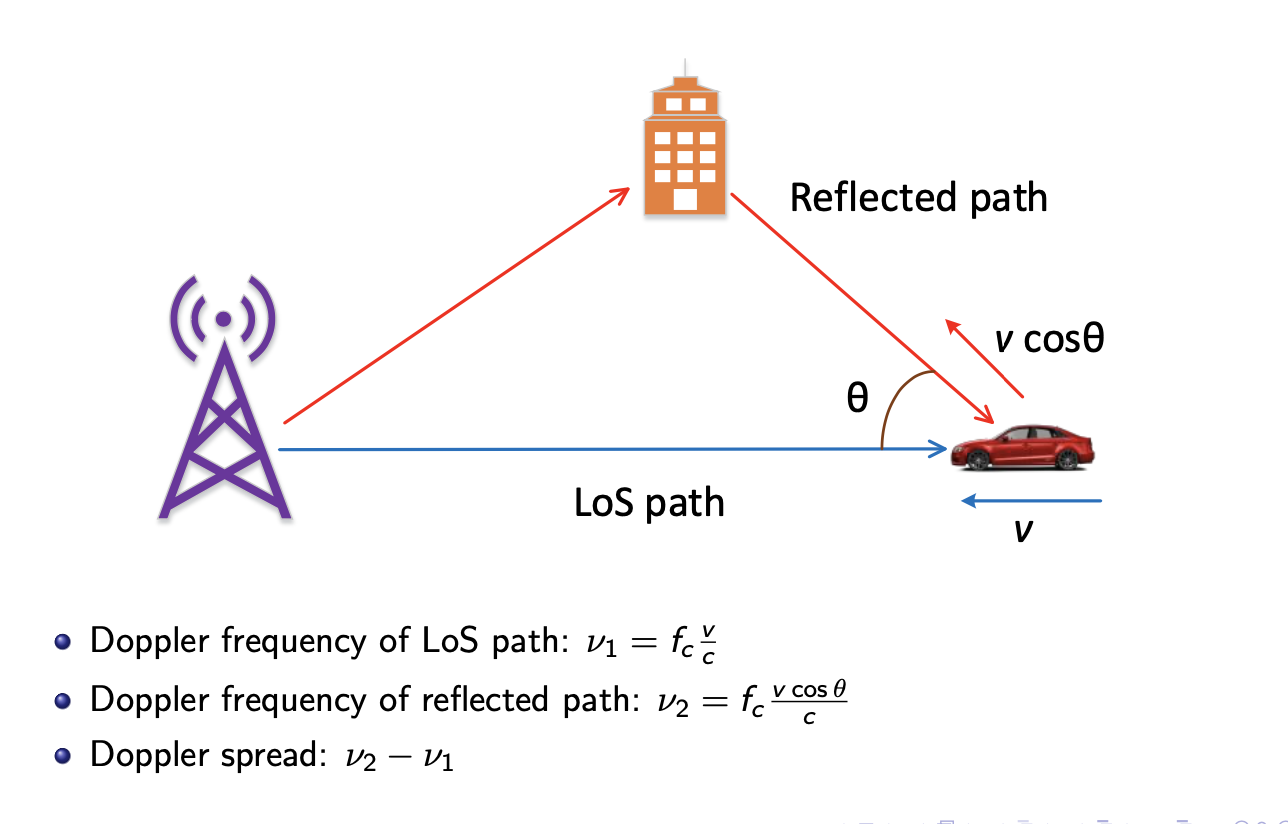
\includegraphics[width=0.82\textwidth]{Images/Chapter2/doppler_spread.png}
    \caption[Illustration of Doppler shift and Doppler spread in a wireless channel.]{Illustration of Doppler shift and Doppler spread in a wireless channel~\protect\cite{Hong2019OTFSTutorial}.}
    \label{fig:doppler_spread}
\end{figure}

Figure~\ref{fig:doppler_spread} illustrates the Doppler effect in a mobile wireless channel. For the LoS path, the motion is assumed to be aligned with the propagation direction, so the Doppler shift can be written as \(f_D=f_c v/c\). For the reflected path, only the velocity component along the propagation direction contributes to the Doppler shift, resulting in \(f_D=f_c v\cos\theta/c\). Since different propagation paths may arrive from different directions, they experience different Doppler shifts.

When multiple propagation paths are present, the received signal contains a range of Doppler shifts rather than a single frequency offset. This range is called Doppler spread. A small Doppler spread means that the channel varies slowly with time, while a large Doppler spread indicates a rapidly time-varying channel.

Doppler spread describes how much the received signal is spread in frequency due to motion. A small Doppler spread means that the channel varies slowly with time. A large Doppler spread means that the channel changes rapidly. Therefore, Doppler spread is closely related to time selectivity.

In low-mobility systems, the wireless channel may remain nearly constant over several symbol intervals. In this case, conventional channel estimation and equalization methods are usually effective. However, in high-mobility environments, the channel may change significantly during a transmission frame or even within one OFDM symbol. This rapid variation makes detection more difficult and may lead to serious performance degradation.

The Doppler effect is particularly important for OFDM systems. OFDM relies on the orthogonality among subcarriers. When the channel varies rapidly due to large Doppler spread, this orthogonality may be destroyed. As a result, energy from one subcarrier leaks into neighboring subcarriers, producing inter-carrier interference (ICI).

Table~\ref{tab:doppler_effects} summarizes the main effects of Doppler shift and Doppler spread.

\begin{table}[H]
\centering
\caption{Effects of Doppler shift and Doppler spread.}
\label{tab:doppler_effects}

\begin{tabular}{|p{4cm}|p{4cm}|p{5cm}|}
\hline
\textbf{Cause} &
\textbf{Channel Effect} &
\textbf{Main Consequence} \\
\hline

Relative motion &
Frequency shift of each path &
Doppler shift \\
\hline

Multiple moving paths &
Range of Doppler shifts &
Doppler spread \\
\hline

Large Doppler spread &
Rapid channel variation &
Time selectivity \\
\hline

Time-selective channel &
Loss of subcarrier orthogonality &
Inter-carrier interference \\
\hline

High mobility &
Fast time-varying channel response &
Difficult channel estimation and equalization \\
\hline

\end{tabular}

\end{table}

In summary, delay spread is mainly associated with multipath propagation, while Doppler spread is mainly associated with mobility. Delay spread causes frequency selectivity, whereas Doppler spread causes time selectivity. Both effects appear simultaneously in many practical high-mobility systems.

\subsubsection{Doubly Selective Channels}

A wireless channel is called doubly selective when it is both frequency selective and time selective. Frequency selectivity is caused by delay spread, while time selectivity is caused by Doppler spread. Therefore, doubly selective channels appear when multipath propagation and mobility occur simultaneously.

Doubly selective channels are common in high-mobility wireless communication scenarios. Examples include high-speed railways, vehicular networks, unmanned aerial vehicles, and low-earth-orbit satellite communications. In these scenarios, the transmitted signal experiences multiple propagation paths and rapid channel variation at the same time.

\begin{figure}[H]
    \centering

    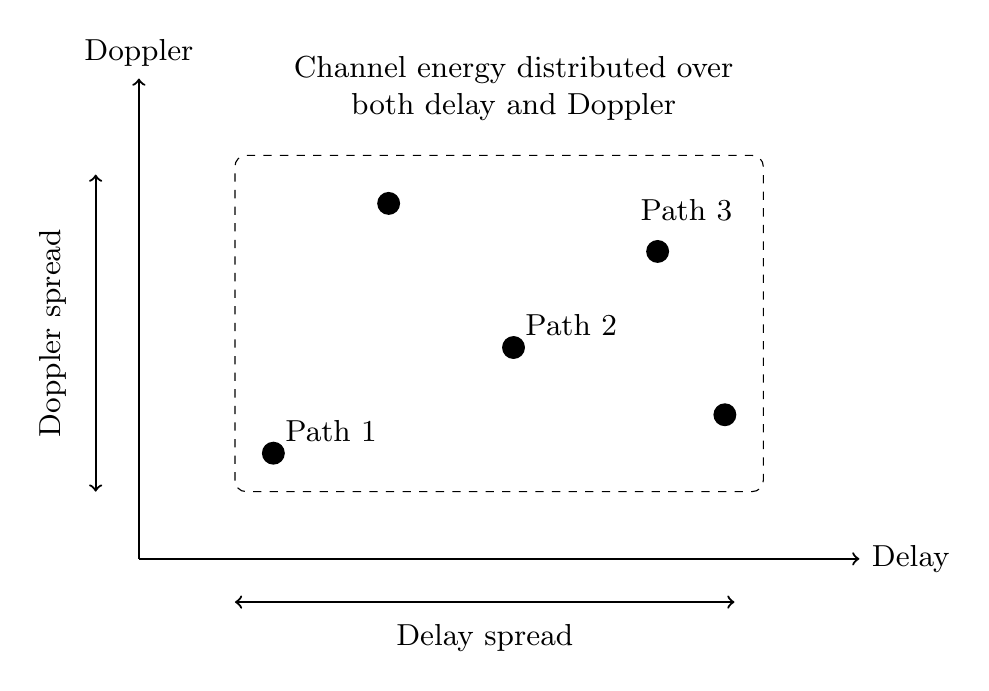
\begin{tikzpicture}[
        scale=1.22,
        transform shape,
        every node/.style={font=\small},
        axis/.style={->, thick},
        pathpoint/.style={circle, fill=black, inner sep=2.4pt},
        spread/.style={draw, dashed, rounded corners}
    ]

    % Axes
    \draw[axis] (0,0) -- (7.5,0) node[right] {Delay};
    \draw[axis] (0,0) -- (0,5.0) node[above] {Doppler};

    % Dashed area showing channel support
    \draw[spread] (1.0,0.7) rectangle (6.5,4.2);

    % Title inside the figure, moved away from y-axis label
    \node[align=center] at (3.9,4.9)
    {Channel energy distributed over\\both delay and Doppler};

    % Delay and Doppler spread indication
    \draw[<->, thick] (1.0,-0.45) -- (6.2,-0.45);
    \node at (3.6,-0.82) {Delay spread};

    \draw[<->, thick] (-0.45,0.7) -- (-0.45,4.0);
    \node[rotate=90] at (-0.9,2.35) {Doppler spread};

    % Path points
    \node[pathpoint] at (1.4,1.1) {};
    \node[pathpoint] at (2.6,3.7) {};
    \node[pathpoint] at (3.9,2.2) {};
    \node[pathpoint] at (5.4,3.2) {};
    \node[pathpoint] at (6.1,1.5) {};

    % Labels
    \node[above right] at (1.4,1.1) {Path 1};
    \node[above right] at (3.9,2.2) {Path 2};
    \node[above right] at (5.1,3.4) {Path 3};

    \end{tikzpicture}

    \caption{Conceptual illustration of a doubly selective channel with both delay and Doppler dispersion.}
    \label{fig:doubly_selective_channel}
\end{figure}

Figure~\ref{fig:doubly_selective_channel} conceptually illustrates a doubly selective channel. The delay dimension represents multipath-induced time dispersion, while the Doppler dimension represents mobility-induced frequency dispersion. Instead of being concentrated around a single propagation component, the channel energy is distributed across both delay and Doppler dimensions.

From a communication system perspective, doubly selective channels are difficult because they introduce both ISI and ICI. Delay spread may cause symbols to overlap in time, leading to ISI. Doppler spread may destroy subcarrier orthogonality, leading to ICI. When both effects are present, receiver design becomes significantly more challenging.

\begin{table}[H]
\centering
\caption{Relationship between propagation effects and channel selectivity.}
\label{tab:channel_selectivity}

\begin{tabular}{|p{4cm}|p{4cm}|p{5cm}|}
\hline
\textbf{Propagation Effect} &
\textbf{Channel Characteristic} &
\textbf{Resulting Impairment} \\
\hline

Delay spread &
Frequency selectivity &
Inter-symbol interference \\
\hline

Doppler spread &
Time selectivity &
Inter-carrier interference \\
\hline

Delay spread and Doppler spread &
Doubly selective channel &
ISI and ICI simultaneously \\
\hline

\end{tabular}

\end{table}

The concept of a doubly selective channel is central to the motivation of OTFS. OFDM can effectively deal with frequency-selective fading when the channel is approximately constant over one OFDM symbol. However, in high-Doppler environments, the channel changes rapidly and the simple diagonal subcarrier model of OFDM is no longer valid. This leads to significant performance degradation.

For this reason, waveform designs for future high-mobility communications must handle both delay and Doppler effects. OTFS addresses this problem by representing information symbols in the delay-Doppler domain, where the wireless channel can often be described more compactly in terms of physical propagation paths. Before discussing OTFS in detail, the next section reviews OFDM, which remains the dominant waveform in current wireless communication systems and provides a useful reference point for understanding the need for OTFS.
